\documentclass[11pt]{article}

%%%%%%%%%%%%%%Include Packages%%%%%%%%%%%%%%%%%%%%%%%%%%
\usepackage{xcolor}
\usepackage{mathtools}
\usepackage[a4paper, total={6in, 8in}, margin=1.25in]{geometry}
\usepackage{amsmath}
\usepackage{amssymb}
\usepackage{paralist}
\usepackage{rsfso}
\usepackage{amsthm}
\usepackage{wasysym}
\usepackage[inline]{enumitem}   
\usepackage{hyperref}
\usepackage{tocloft}
\usepackage{titlesec}
\usepackage{colortbl}
\usepackage{wrapfig}
\usepackage{pdfpages}
%%%%%%%%%%%%%%%%%%%%%%%%%%%%%%%%%%%%%%%%%%%%%%%%%%%%%%%%



\begin{document}
\Large \noindent \textbf{Physics 5A Discussion (Week 6)}\\
\normalsize
Department of Physics and Astronomy, UCLA\\
\noindent\rule{8cm}{0.4pt}\\
\begin{center}
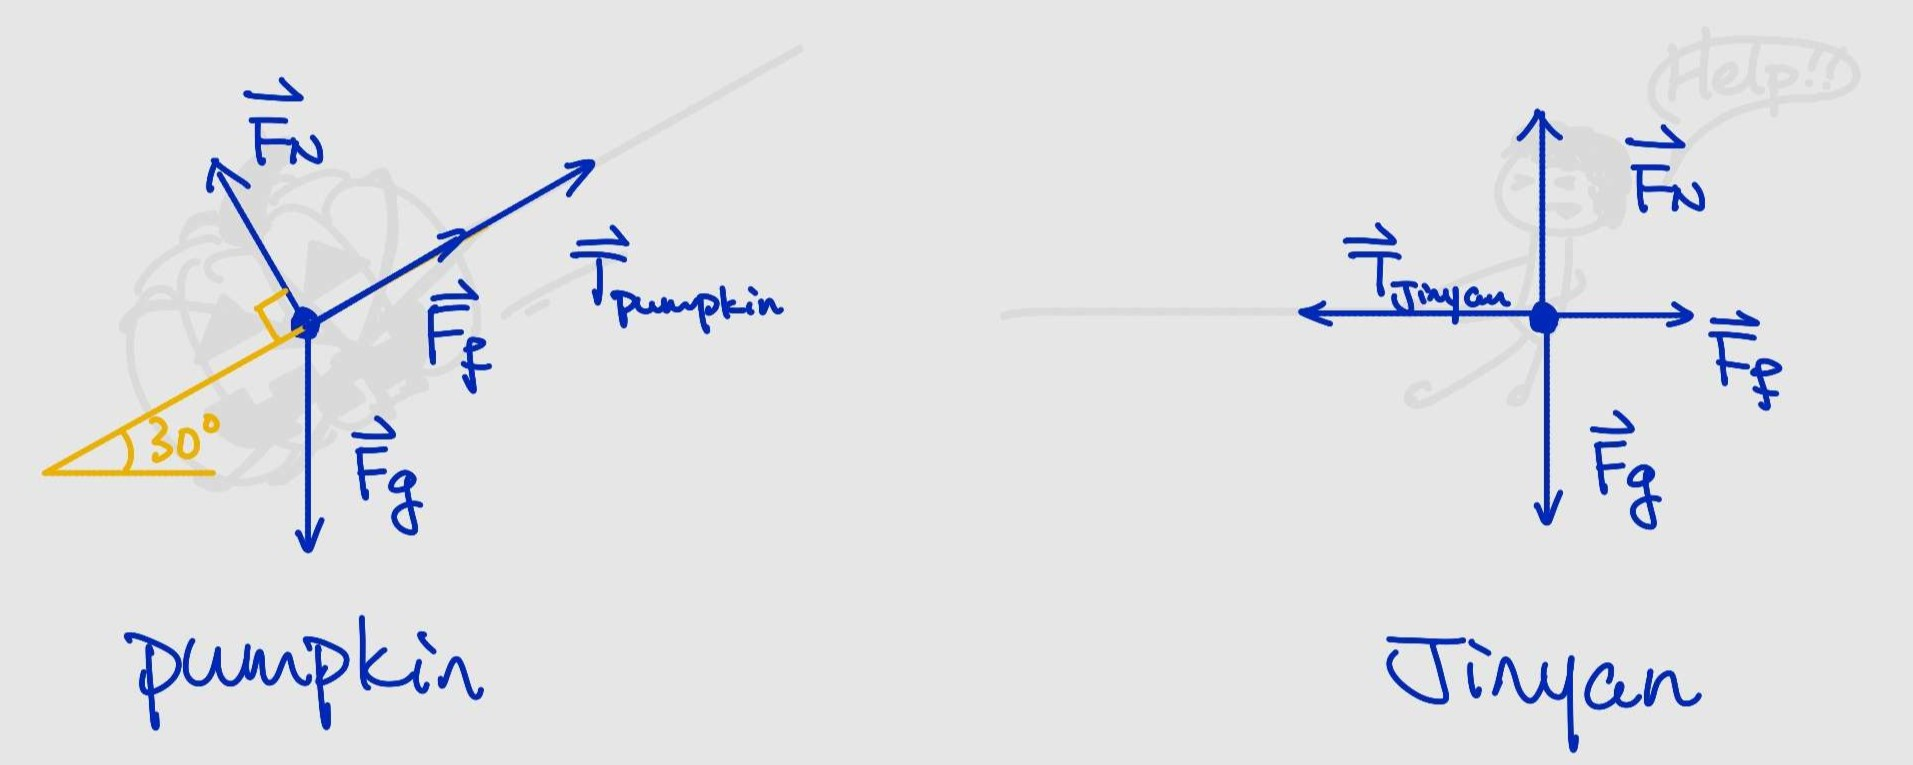
\includegraphics[scale=0.55]{pull}
\end{center}
Jinyan on the hill is trying to pull the pumpkin uphill. However, the pumpkin is so heavy that it makes Jinyan slip to the left, with an acceleration $\vec{a}$ as shown. Simultaneously, the pumpkin is slipping down the hill with an acceleration $\vec{a}'$. The coefficient of kinetic friction of the surface is $\mu_k = 0.1$, and the masses of Jinyan and the gigantic pumpkin are both $60\,$kg. Find the acceleration $\vec{a}$, and the force $\vec{T}$ that Jinyan applies to pull the cord.\\

\noindent\textbf{Step 1:} Draw the free-body diagrams for Jinyan and the pumpkin, you don't need to compute the magnitudes of the forces yet, just indicate their directions. (\textit{Hint: Gravity, friction, normal force, and tension.})\\

\noindent Pumpkin: \qquad\qquad\qquad\qquad\qquad\qquad\qquad
Jinyan:
\hfill\break\hfill\break\hfill\break
\hfill\break\hfill\break\hfill\break


\noindent \textbf{Step 2:} Compute the gravitational force $\vec{F}_g$ and normal force $\vec{F}_N$ acting on Jinyan. (\textit{Hint: They should cancel exactly, as Jinyan is not moving up or down.})\\
\hfill\break\hfill\break\hfill\break

\noindent \textbf{Step 3:} Compute the kinetic friction $\vec{F}_f$ that Jinyan experiences. \\
\hfill\break\hfill\break\hfill\break

\noindent \textbf{Step 4:} Recall what we have done last week, compute the gravitational force and normal force acting on the pumpkin, in $\parallel$- and $\perp$-components. (\textit{Hint: The $\perp$-component of the gravitational force cancels the normal force}.)

\newpage
\noindent \textbf{Step 5:} Compute the kinetic friction experienced by the pumpkin. 
\hfill\break\hfill\break\hfill\break

\noindent \textbf{Step 6:} We know that the net force acting on Jinyan should point in the horizontal direction (because Jinyan is not moving up or down), so
$$F_{\text{net force on Jinyan},\,x} = -ma\,.$$
Find the left-hand side of this equation in terms of $T_{\text{Jinyan}}$ (the magnitude of the force that Jinyan is pulling on the cord). \\
\hfill\break\hfill\break\hfill\break
\hfill\break\hfill\break\hfill\break

\noindent \textbf{Step 7:} The net force on the pumpkin has only the parallel component, so 
\begin{align*}
F_{\text{net force on pumpkin},\, \parallel} = -ma'\,.
\end{align*} 
Find the left-hand side of this equation in terms of $T_{\text{pumpkin}}$ (the magnitude of the force that the pumpkin is pulling on the cord).
\hfill\break\hfill\break\hfill\break
\hfill\break\hfill\break\hfill\break

\noindent \textbf{Step 8:} We have $a = a'$ and $T_{\text{Jinyan}}=T_{\text{pumpkin}}$ (why?). Then we can set 
\begin{align*}
F_{\text{net force on pumpkin},\, \parallel} = F_{\text{net force on Jinyan},\,x}
\end{align*}
You should be able to find the tension $T = T_{\text{Jinyan}}$ from here.\\
\hfill\break\hfill\break\hfill\break
\hfill\break\hfill\break\hfill\break
\hfill\break\hfill\break\hfill\break

\noindent \textbf{Step 9:} Using $\vec{F}_{\text{net}} = m\vec{a}$ to find $\vec{a}$. 


%\noindent Part (b) as an exercise: Under such a scenario, how long does it take for the pumpkin to pull Jinyan to the left by $1$ meter? How far in the downhill direction does the pumpkin move in this time period?
\newpage
\noindent Solutions:\\

\textbf{Step 1}:\\
\begin{center}
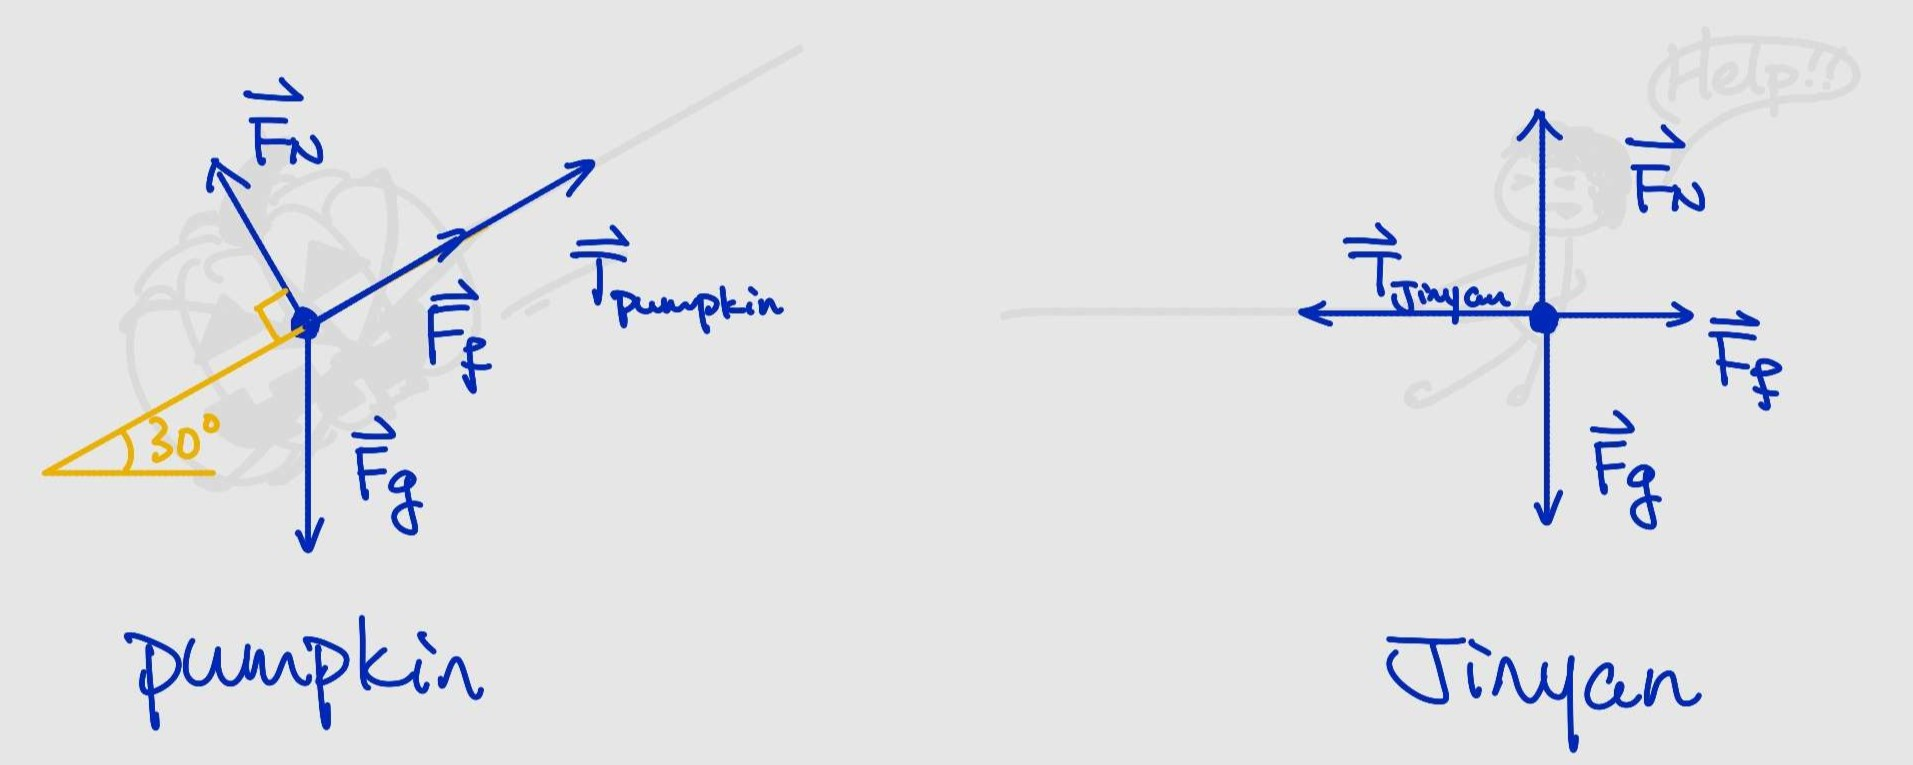
\includegraphics[scale=0.25]{pull.jpg}
\end{center}

\textbf{Step 2}: The gravitational force points straight down. The normal force cancels the perpendicular component of the gravitational force, pointing in a direction perpendicular to the surface. For Jinyan, we have
\begin{align*}
&\vec{F}_g = m \vec{g} = (60\,\text{kg})\cdot \left((0 \hat{\i} -9.8\hat{\j})\,\text{m/s}^2 \right) = \left(0\hat{\i}-588\hat{\j}\right)\,\text{N}\,,\qquad\vec{F}_N  = \left(0\hat{\i}+588\hat{\j}\right)\,\text{N}\,.
\end{align*}

\textbf{Step 3:} Friction on Jinyan is calculated from the normal force, 
\begin{align*}
\vec{F}_f = \left(\mu_k F_N\,\hat{\i} + 0\hat{\j}\right) \,\text{N} = \left( 58.8\hat{\i}+0\hat{\j}\right) \,\text{N}\,.
\end{align*}
The $x$-component is positive because friction points directly to the right.\\

\textbf{Step 4:} We have done in last week a similar decomposition for the gravitational force acting on the pumpkin. For the details, check the week-5 worksheet, 
\begin{align*}
\vec{F}_g = \left( -mg\sin(30^\circ)\hat{\i}-mg\cos(30^\circ)\hat{\j}\right)\,\text{N}= \left( -588\sin(30^\circ)\hat{\i}-588\cos(30^\circ)\hat{\j}\right)\,\text{N}
\end{align*}
The negative signs indicate the direction of the parallel (downhill) and perpendicular (into-the-incline) components of the gravitational force on the pumpkin. The normal force on the pumpkin only cancels the perpendicular component of the gravitational force, in order to prevent the pumpkin from moving into the incline, thus
\begin{align*}
\vec{F}_N =\left( 0+588\cos(30^\circ)\hat{\j}\right)\,\text{N}\,.
\end{align*}

\textbf{Step 5:} Now the friction on the pumpkin is calculated from the normal force on the pumpkin. It is pointing in the uphill direction as it opposes the direction of motion of the pumpkin, which is slipping down the hill, 
\begin{align*}
\vec{F}_f = \left(\mu_k F_N\,\hat{\i} + 0\hat{\j}\right) \,\text{N} = \left( 58.8\cos(30^\circ)\hat{\i}+0\hat{\j}\right) \,\text{N}\,,
\end{align*}
written in $(\parallel$,$\perp)$-component form. \\


\textbf{Step 6:} Now we want to find the net force acting on Jinyan, all the $y$-components are canceled, so we only need to take care of the $x$-components, 
\begin{align*}
F_{\text{net force on Jinyan},\,x} =58.8 -T =-ma\,. 
\end{align*}
where $T$ is the magnitude of the tension, and $a$ is the magnitude of the acceleration. The negative sign in front of $ma$ indicates that the acceleration is leftward. The negative sign in front of $T$ indicates that the cord is pulling Jinyan to the left.\\

\textbf{Step 7:} For the net force acting on the pumpkin, we first notice that all the perpendicular components are canceled (the $\perp$-component of the normal force cancels with the $\perp$-component of the gravitational force, friction and tension have no $\perp$-component as seen from the free-body diagram), so we only need to take care of the parallel components, 
\begin{align*}
F_{\text{net force on pumpkin},\, \parallel} =-588\sin(30^\circ) + 58.8\cos(30^\circ)+T =-ma'\,.
\end{align*}
Again, the signs are important. The negative sign in front of $ma'$ indicates that the pumpkin is sliding downhill.\\

\textbf{Step 8:} We realize $a=a'$ because the pumpkin and Jinyan should move together, with the same acceleration and speed, because they are ``connected" by the cord. Tension of an ideal cord is the same everywhere (this is a general assumption), so we write
\begin{align*}
F_{\text{net force on Jinyan},\,x} &= F_{\text{net force on pumpkin}\,, \parallel}\\
58.8 -T &=-588\sin(30^\circ) + 58.8\cos(30^\circ)+T\\
T&= 150.9\,\text{N}
\end{align*}
which is the magnitude of the tension. For the tension vector, when acting on Jinyan, 
\begin{align*}
\vec{T}_{\text{Jinyan}} = \left(-150.9\hat{\i}+0\hat{\j}\right)\,\text{N}  
\end{align*}
with the negative sign indicating it is pulling Jinyan to the left. When acting on the pumpkin,
\begin{align*}
\vec{T}_{\text{pumpkin}} = \left(150.9\hat{\i}+0\hat{\j}\right)\,\text{N}  \,,
\end{align*}
indicating that it is pulling the pumpkin uphill.\\

\textbf{Step 9:} To find $a$, we use 
\begin{align*}
F_{\text{net force on Jinyan},\,x} =58.8 -T=58.8-150.9 =-ma = -60a\,,
\end{align*}
so we see that 
\begin{align*}
a = 1.53\,\text{m/s}^2\,.
\end{align*}
The actual Jinyan's acceleration vector should be pointing to the left, 
\begin{align*}
\vec{a} = \left(-1.53\hat{\i}+0\hat{\j}\right)\,\text{m/s}^2\,.
\end{align*}

\end{document}


